
\section{使用部品の選定(TWELITE)}

基本設計の段階において,筆者が担当した室外デバイスで使用する部品の選定を行った.
室外デバイスのマイコンについては,モノワイヤレス株式会社の無線マイコンであるTWELITEを使用した\cite{twelite}.
室外デバイスはJetsonと通信する必要があり,また,コードの配線を考えずに済むように無線通信ができるマイコンを採用することとした.
さらに設置場所の制約を少なくするため,室外デバイスはできるだけサイズを小さくしたい.このため,マイコンボードに無線機能があらかじめ実装されているもの,乾電池で動作できるものを採用することとした.ただし,乾電池の一般的な起電力である1.5Vで動作するマイコンボードはほとんどないため,ここでは乾電池を2本使用して3Vで動作するものとする.
以上の理由より,起電力3Vで動作し,無線機能があらかじめ実装されているTWELITEを選定した.
今回使用したのはTWELITE DIP BLUEである(図\ref{tweblue}).以下の表\ref{siyou}に仕様を示す.

\begin{figure}
	\centering
	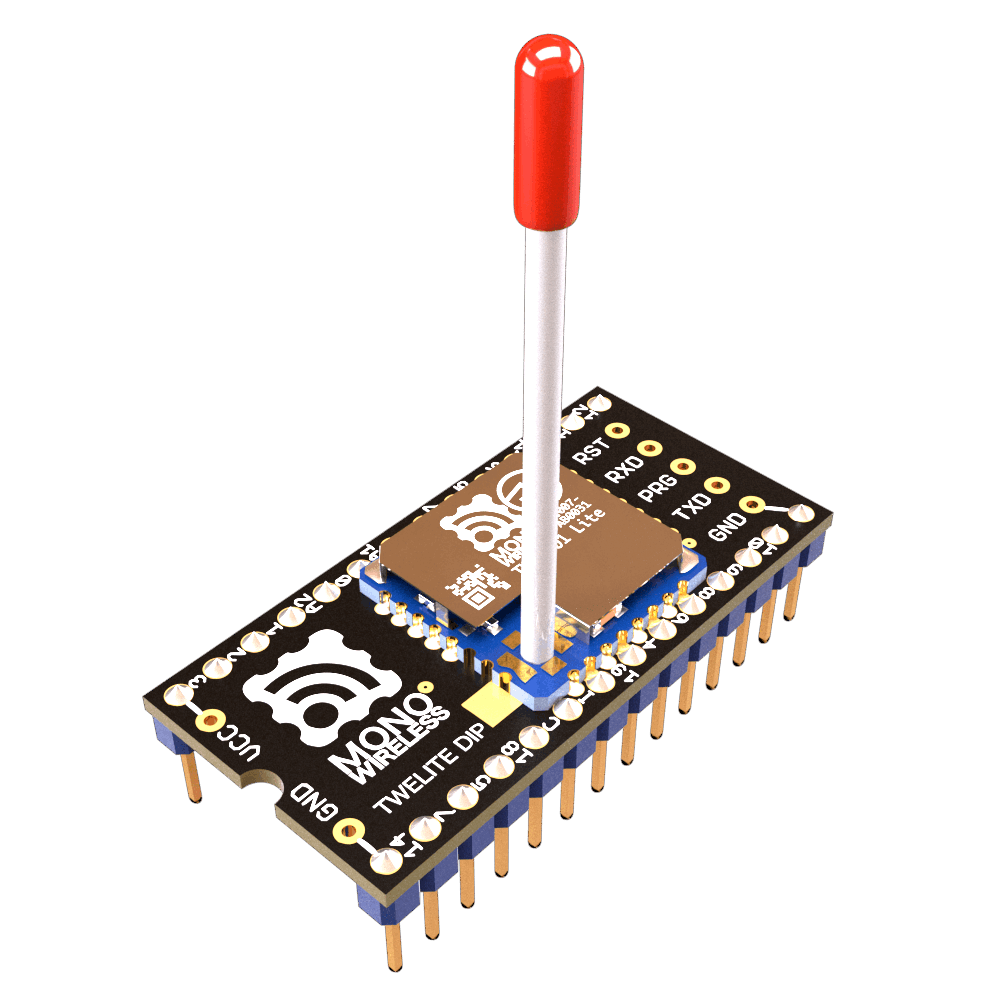
\includegraphics[width=0.3\linewidth]{tweblue}
	\caption{TWELITE DIP BLUE}
	\label{tweblue}
\end{figure}

\begin{table}
	\centering
	\caption{TWELITE DIP BLUEの仕様}
	\begin{tabular}{|c|c|}
		\hline
		送信出力 & +2.50dBm \\
		\hline
		受信感度 & -95dBm \\
		\hline
		送信電流 & 15.3mA (+2.50dBm出力時) \\
		\hline
		受信電流 & 17.0mA \\
		\hline
		外形寸法 & 35.7mm x 17.7mm x 3.5mm \\
		
		& (アンテナ,コネクタ,端子除く) \\
		\hline
		& 3.6g (マッチ棒アンテナ版) \\
		
		重量 & 3.7g (同軸コネクタ版) \\
		
		& (アンテナ,コネクタ,端子除く) \\
		\hline
		動作電圧 & 2.3~3.6V \\
		\hline
		動作温度 & -40~85℃ \\
		\hline
		電波認証 & ARIB STD-T66 (技適) \\
		\hline
	\end{tabular}
	\label{siyou}
\end{table}
\newpage